\documentclass{llncs}
\usepackage{times}
\usepackage[T1]{fontenc}

% Comentar para not MAC Users
%\usepackage[applemac]{inputenc}
\usepackage[utf8]{inputenc}
\usepackage[portuguese]{babel}
\usepackage{a4}
%\usepackage[margin=3cm,nohead]{geometry}
\usepackage{epstopdf}
\usepackage{graphicx}
\usepackage{fancyvrb}
\usepackage{amsmath}
\usepackage{subcaption}
\usepackage{tikz}
\usepackage[bookmarks=false]{hyperref}
\usepackage{float}
%\renewcommand{\baselinestretch}{1.5}

\newcommand{\questionE}[1]{\textcolor{gray}{\textit{"#1"}}}

\begin{document}
\mainmatter
\title{TP2: Protocolo IPv4}

\titlerunning{TP2: Protocolo IPv4}

\author{Sérgio Jorge \and João Freitas \and Alexandre Martins}

\authorrunning{Sérgio Jorge \and João Freitas \and Alexandre Martins}


\institute{
University of Minho, Department of  Informatics, 4710-057 Braga, Portugal\\
e-mail: \{a77730,a74814,a77523\}@alunos.uminho.pt
}

\date{}
\bibliographystyle{splncs}

\maketitle
\section{Introdução}
\hspace{3mm} 

O principal objetivo deste trabalho é o aprofundamento de conhecimentos em protocolo IPv4 através do estudo do formato de um pacote/datagrama IP, fragmentação de pacotes IP e endereçamento e encaminhamento IP, utilizando ferramentas como \textit{Wireshark}, \textit{PingPlotter}, \textit{TraceRoute}, \textit{NetStat} e \textit{CORE}. 

\clearpage

\section{Grupo I - Parte 1}

\begin{figure}[H]
\begin{center}
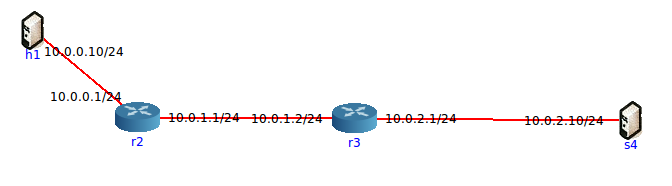
\includegraphics[width=12cm]{topo1.PNG}
\end{center}
\caption{Topologia Inicial}
\end{figure}

\subsection{Questão A}
\hspace{3mm} 
\questionE{Active o wireshark ou o tcpdump no pc h1. Numa shell de h1, execute o comando traceroute -I para o endereço IP do host s4.}\\ 

\begin{figure}[H]
\begin{center}
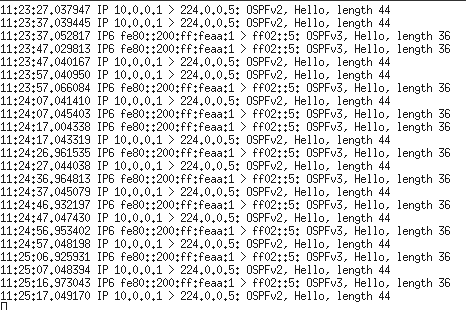
\includegraphics[width=10cm]{1aTracedump.PNG}
\end{center}
\caption{\textit{TCPDump} no pc h1}
\end{figure}

\begin{figure}[H]
\begin{center}
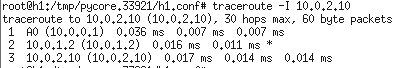
\includegraphics[width=10cm]{1aTraceroute.PNG}
\end{center}
\caption{\textit{Traceroute} no host s4}
\end{figure}

\subsection{Questão B}
\hspace{3mm}
\questionE{Registe e analise o tráfego ICMP enviado por h1 e o tráfego ICMP recebido como resposta. Comente os resultados face ao comportamento esperado.}\\

Como se pode observar na figura 4, temos varias sequências de \textit{ICMP echo request} com a resposta correspondente \textit{ICMP echo reply}. Pode-se também observar que a resposta do host s4 falha na 6ª sequência, daqui assumimos que o Time-To-Live (TTL) era menor que o número de saltos necessários para a ligação. Como na sequência 7 já se obteve resposta do host s4 e o TTL vai sendo incrementado em uma unidade para se descobrir qual o mínimo necessário, então, aqui, conclui-se que já é suficiente para efetuar a ligação com sucesso entre h1 e s4. Daí em diante, todas as tentativas de ligação obtém resposta com sucesso.

\begin{figure}[H]
\begin{center}
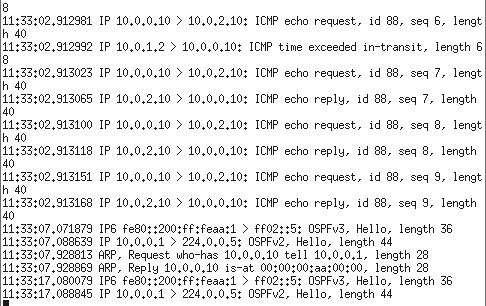
\includegraphics[width=10cm]{1b.PNG}
\end{center}
\caption{Tráfego ICMP - entre h1 e s4}
\end{figure}

\subsection{Questão C}
\hspace{3mm}
\questionE{Qual deve ser o valor inicial mínimo do campo TTL para alcançar o destino s4? Verifique na prática que a sua resposta está correta.}\\

O valor inicial mínimo do campo TTL tem de ser 3, visto que o número de saltos é 3 (h1->r2; r2->r3; r3->s4).

Além disso, na parte 2 da figura 5, procurou-se limitar o número de saltos em 3, e o destino foi alcançado na mesma. 

\begin{figure}[H]
\begin{center}
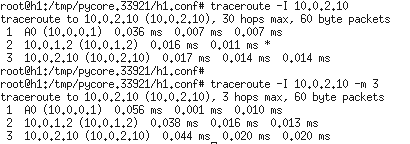
\includegraphics[width=10cm]{1c.PNG}
\end{center}
\caption{\textit{Traceroute} entre h1 e s4}
\end{figure}

\subsection{Questão D}
\hspace{3mm}
\questionE{Qual o valor médio do tempo de ida-e-volta (Round-Trip Time) obtido?}\\

O valor médio do tempo ida-e-volta é 0.028ms, obtido através da média da terceira linha da Figura 5, somando os três tempos dados pelo terceiro salto e dividindo por 3.


\clearpage

\section{Grupo II - Parte 1}

\subsection{Questão A}
\hspace{3mm} 
\questionE{Qual é o endereço IP da interface ativa do seu computador?}\\

O endereço de IP da interface ativa é 192.168.2.190.

\subsection{Questão B}
\hspace{3mm}
\questionE{Qual é o valor do campo protocolo? O que identifica?}\\

O valor do campo protocolo é ICMP, \textit{Internet Control Message Protocol}. Este protocolo é utilizado para reportar e gerir erros na rede. Ou seja, a partir dele, um \textit{router} ou um host pode mencionar à origem que houve um erro no processamento do datagrama. Por exemplo: 

\begin{itemize}
    \item \textit{time exceeded message} - quando o TTL chega a 0 e o datagrama tem de ser descartado;
    
    \item \textit{echo request/reply} - mensagens enviadas para teste ou controlo da rede (\textit{request}); se a máquina destino está disponível, então responde (\textit{reply});
    
    \item \textit{destination unreachable} - quando não se consegue alcançar o destino; 
\end{itemize}

É, também, um protocolo que funciona ao nível de rede e, por isso, as mensagens são encapsuladas em datagramas IP.

\begin{figure}[H]
\begin{center}
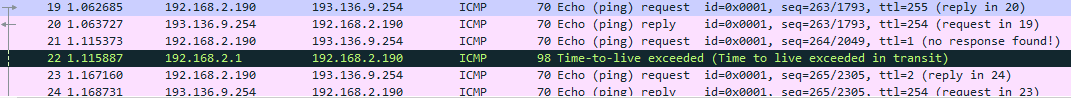
\includegraphics[width=12cm]{2b.png}
\end{center}
\caption{Primeiras mensagens ICMP}
\end{figure}

\subsection{Questão C}
\hspace{3mm}
\questionE{Quantos bytes tem o cabeçalho IP(v4)? Quantos bytes tem o campo de dados (payload) do datagrama? Como se calcula o tamanho do payload?}\\

Verifica-se que o \textit{header} do datagrama tem 20 bytes e no total, este tem 56 bytes. Por isso, fazendo 56-20 chega-se ao tamanho do \textit{payload} que tem então 36 bytes.

\begin{figure}[H]
\begin{center}
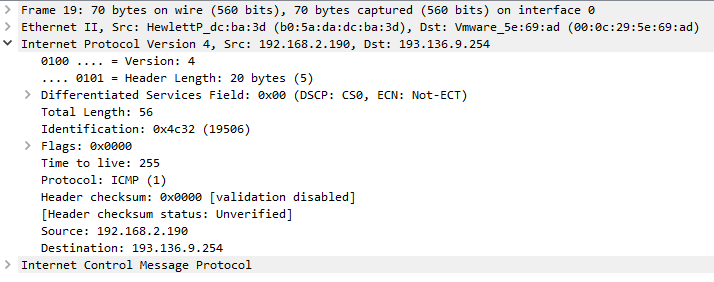
\includegraphics[width=10cm]{2c.PNG}
\end{center}
\caption{Datagrama IP}
\end{figure}

\subsection{Questão D}
\hspace{3mm}
\questionE{O datagrama IP foi fragmentado? Justifique.}\\

A fragmentação surge quando um datagrama excede o MTU (Maximum Tranfer Unit).
Como a flag \textit{More Fragments} tem o valor \textit{Not Set} e o \textit{Fragment offset} é 0, podemos assumir que o datagrama IP não foi fragmentado. Ou seja, conclui-se que o MTU é superior ao tamanho do datagrama.

\begin{figure}[H]
\begin{center}
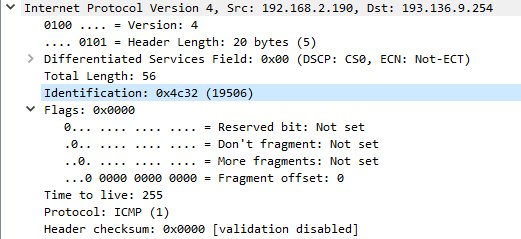
\includegraphics[width=10cm]{2d.PNG}
\end{center}
\caption{}
\end{figure}

\clearpage

\subsection{Questão E}
\hspace{3mm}
\questionE{Ordene os pacotes capturados de acordo com o endereço IP fonte (e.g., selecionando o cabeçalho da coluna \textit{Source}), e analise a sequência de tráfego ICMP gerado a partir do endereço IP atribuído à interface da sua máquina. Para a sequência de mensagens ICMP enviadas pelo seu computador,	indique que campos do cabeçalho IP variam de pacote para pacote.}\\

Os campos do cabeçalho IP que variam são a identificação e o time-to-live (TTL).

A identificação muda porque identifica unicamente cada datagrama.

O TTL muda porque a máquina tenta ligar-se ao destino, começando com um TTL = 1. Quando o pacote é descartado, esta percebe que tem de incrementar o TTL até alcançar o destino. 


\begin{figure}[H]
\begin{center}
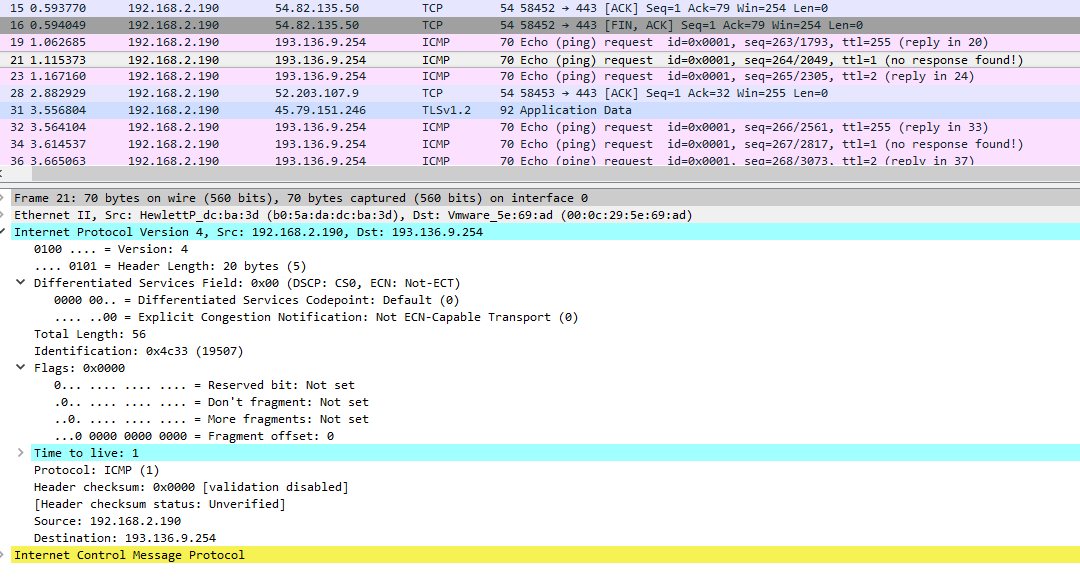
\includegraphics[width=12cm]{2ef.PNG}
\end{center}
\caption{Tráfego ICMP}
\end{figure}

\subsection{Questão F}
\hspace{3mm}
\questionE{Observa algum padrão nos valores do campo de Identificação do datagrama IP e TTL?}\\

O campo identificação muda, incrementando por um, e o campo Time-To-Live (TTL) começa em 255 porque este é o valor \textit{default} em Linux. De seguida, vai testando quantos hops (saltos) são necessários para chegar ao destino, começando com  TTL igual a 1 que dá a mensagem de erro \textit{no response found!} e, de seguida, o TTL é incrementado para 2. Verifica-se, neste ponto, que já é possível alcançar o destino. Caso tal não acontecesse, o TTL continuaria a incrementar até saber o número de saltos mínimo para conseguir ligar-se ao destino.

\begin{figure}[H]
\begin{center}
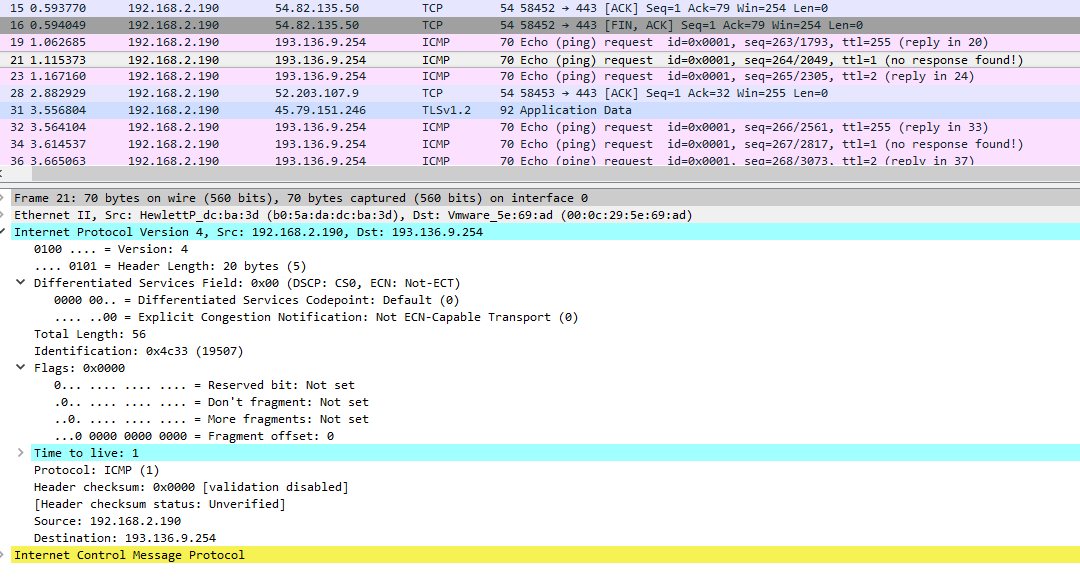
\includegraphics[width=12cm]{2ef.PNG}
\end{center}
\caption{Tráfego ICMP}
\end{figure}

\subsection{Questão G}
\hspace{3mm}
\questionE{Ordene o tráfego capturado por endereço destino e encontre a série de respostas ICMP TTL exceeded enviadas ao seu computador. Qual é o valor do campo TTL? Esse valor permanece constante para todas as mensagens de resposta ICMP TTL exceeded enviados ao seu host? Porquê?}\\

O valor do campo Time-To-Live (TTL) é 64 visto que é o valor \textit{default} da máquina destino e permanece constante entre todas as mensagens de resposta \textit{ICMP TTL exceeded}. Por defeito, quando o \textit{router} desconhece a distância ao host de destino, usa um TTL igual a 64, valor exageradamente alto, de forma a garantir a entrega do datagrama.

\begin{figure}[H]
\begin{center}
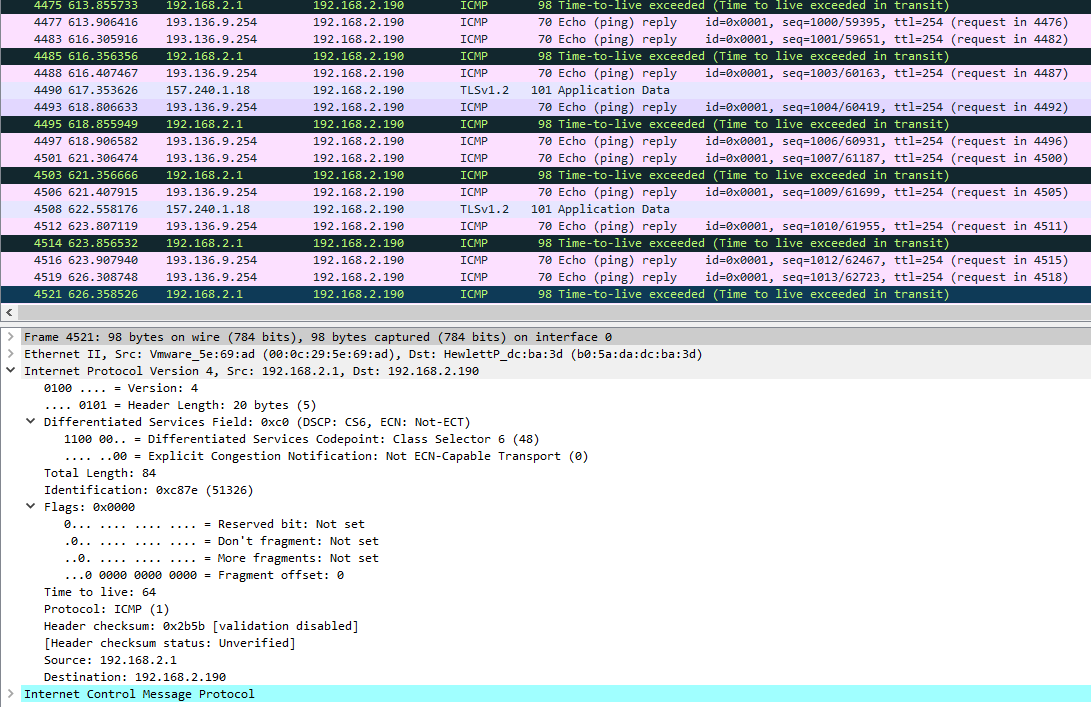
\includegraphics[width=10cm]{2g.PNG}
\end{center}
\caption{Tráfego ICMP}
\end{figure}

\clearpage

\section{Grupo III - Parte 1}

\subsection{Questão A}
\hspace{3mm} 
\questionE{Localize a primeira mensagem ICMP. Porque é que houve necessidade de fragmentar o pacote inicial?}\\ 

Houve necessidade de fragmentar o pacote inicial porque este tem 3565 bytes de tamanho e excede o \textit{Maximum Transmission Unit} (MTU) que é 1500 bytes.

\subsection{Questão B}
\hspace{3mm}
\questionE{Imprima o primeiro fragmento do datagrama IP segmentado. Que informação no cabeçalho indica que o datagrama foi fragmentado? Que informação no cabeçalho IP indica que se trata do primeiro fragmento? Qual é o tamanho deste datagrama IP?}\\

Através da \textit{flag} \textit{More Fragments} que está assinalada a 1 e tem o valor \textit{Set}, podemos afirmar que o datagrama foi fragmentado. Como o \textit{Fragment offset} neste fragmento é 0 concluímos que se trata do primeiro fragmento. O tamanho deste datagrama é 1500 bytes, sendo que 20 destes bytes são para o \textit{header} e 1480 para o \textit{payload}.

\begin{figure}[H]
\begin{center}
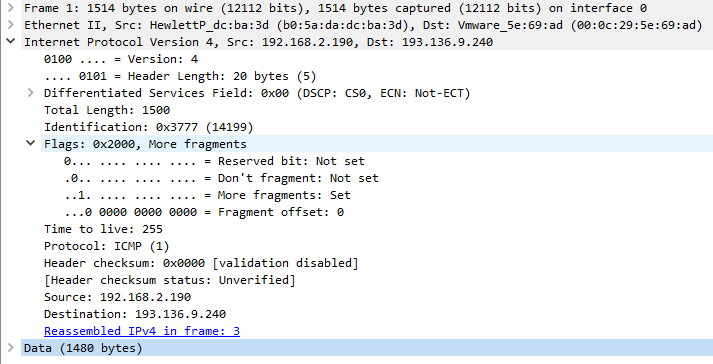
\includegraphics[width=10cm]{3bfragmento1.PNG}
\end{center}
\caption{Fragmento 1}
\end{figure}

\subsection{Questão C}
\hspace{3mm} 
\questionE{Imprima o segundo fragmento do datagrama IP original. Que informação do cabeçalho IP indica que não se trata do 1º fragmento? Há mais fragmentos? O que nos permite afirmar isso?}\\ 

Contrariamente ao primeiro fragmento, o \textit{Fragment offset} deste tem o valor 185, o que indica que não se trata do primeiro. Podemos afirmar que existem mais fragmentos porque a \textit{flag} \textit{More Fragments} está assinalada a 1 e tem o valor \textit{Set}.

\begin{figure}[H]
\begin{center}
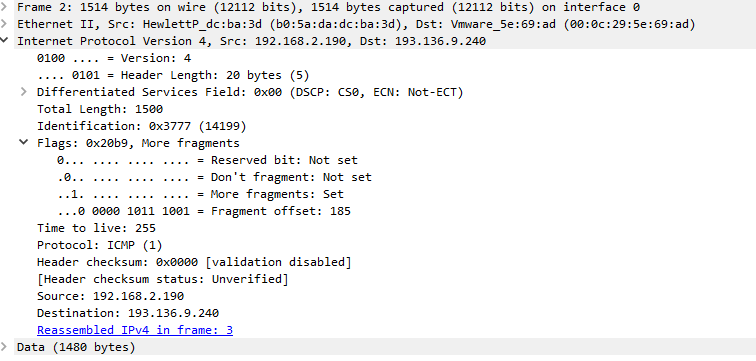
\includegraphics[width=10cm]{3cfragmento2.PNG}
\end{center}
\caption{Fragmento 2}
\end{figure}

\subsection{Questão D}
\hspace{3mm}
\questionE{Quantos fragmentos foram criados a partir do datagrama original? Como se detecta o último fragmento correspondente ao datagrama original?}\\

Foram criados 3 fragmentos, como se pode observar na figura 14. Para detetar o último fragmento do datagrama original procurou-se pelo fragmento no qual o valor da \textit{flag} \textit{More Fragments} estava definido como \textit{Not set}. 

\begin{figure}[H]
\begin{center}
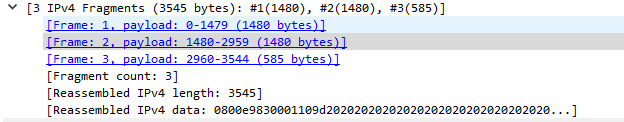
\includegraphics[width=10cm]{3d.PNG}
\end{center}
\caption{Fragmentos criados}
\end{figure}

\begin{figure}[H]
\begin{center}
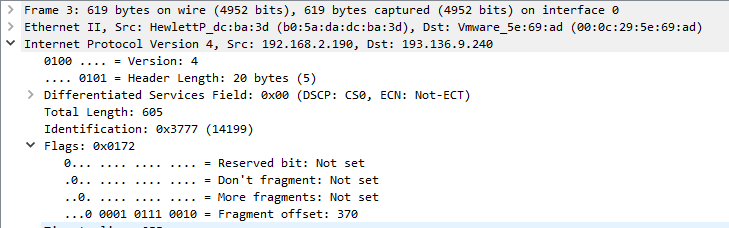
\includegraphics[width=10cm]{3dFrame3temMoreFragmentsA0.PNG}
\end{center}
\caption{Último fragmento}
\end{figure}

\clearpage

\subsection{Questão E}
\hspace{3mm}
\questionE{Indique, resumindo, os campos que mudam no cabeçalho IP entre os diferentes fragmentos, e explique a forma como essa informação permite reconstruir o datagrama original.}\\

Tanto o primeiro como o segundo fragmento têm a mesma \textit{flag} \textit{More Fragments} assinalada a 1 e com o valor \textit{Set}. Também o tamanho destes dois fragmentos é igual, 1500 bytes, que é o tamanho da \textit{Maximum Transmission Unit} (MTU), valor que não pode ser excedido. No terceiro fragmento a \textit{flag} \textit{More Fragments} deixa de estar assinalada a 1, passando a 0, e deixa também de ter o valor \textit{Set}, ficando com \textit{Not Set}. Aqui, o tamanho deixa de ser 1500 bytes pois a informação deste fragmento é inferior à MTU. O campo que muda nos três fragmentos é o campo \textit{Fragment offset} e é este que nos permite reconstruir o datagrama original juntando todos os fragmentos.

\clearpage

\section{Grupo I - Parte 2}

\subsection{Questão A}
\hspace{3mm} 
\questionE{Indique que endereços IP e máscaras de rede foram atribuídos pelo CORE a cada equipamento. Para simplificar, pode incluir uma imagem que ilustre de forma clara a topologia definida e o endereçamento usado.}\\

\begin{figure}[H]
\begin{center}
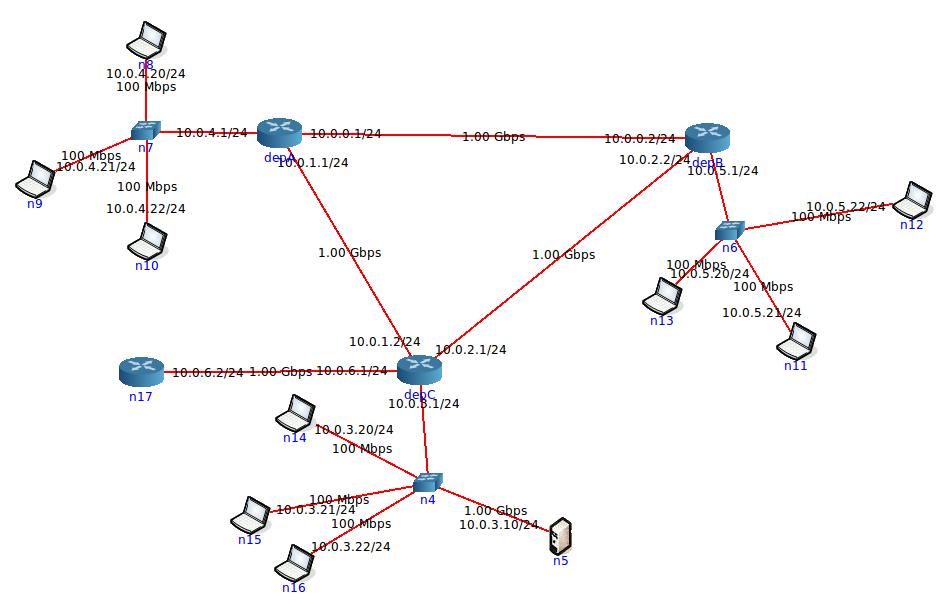
\includegraphics[width=12cm]{topoParteB.jpg}
\end{center}
\caption{Topologia da rede}
\end{figure}

A máscara de rede utilizada é 255.255.255.0 uma vez que os \textit{routers} da rede e os hosts da rede têm endereços /24 atribuídos, ou seja, nestes endereços, 24 bits dos 32 totais identificam a rede.

\subsection{Questão B}
\hspace{3mm}
\questionE{Tratam-se de endereços públicos ou privados? Porquê?}\\

Em redes, o seguinte conjunto de endereços corresponde a endereços privados:

\begin{itemize}
    \item 10.0.0.0 até 10.255.255.255
    \item 172.16.0.0 até 172.31.255.255 
    \item 192.168.0.0 até 192.168.255.255 
    \item 169.254.0.0 até 169.254.255.255
\end{itemize}

Por observação da topologia e dos endereços atribuídos pelo CORE e com o conhecimento acima descrito, é possível afirmar que trata-se de endereços privados.

\subsection{Questão C}
\hspace{3mm}
\questionE{Porque razão não é atribuído um endereço IP aos switches?}\\

Os \textit{switches} não operam ao nível de rede e, por isso, a camada de rede (neste caso, o IP), é completamente transparente para este tipo de dispositivos. Fazem apenas \textit{forward} do pacote para o host destino.

\subsection{Questão D}
\hspace{3mm}
\questionE{Usando o comando ping certifique-se que existe conectividade IP entre os laptops dos vários departamentos e o servidor do departamento C (basta	certificar-se da conectividade de um laptop por departamento).}\\

\begin{figure}[H]
\begin{center}
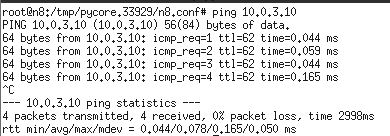
\includegraphics[width=9cm]{PARTEB_1d_n8TOsv.PNG}
\end{center}
\caption{Teste de conectividade entre departamento A e o servidor}
\end{figure}

\begin{figure}[H]
\begin{center}
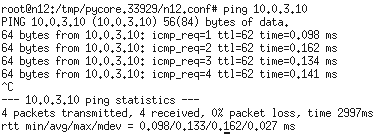
\includegraphics[width=9cm]{PARTEB_1d_n12TOsv.PNG}
\end{center}
\caption{Teste de conectividade entre departamento B e o servidor}
\end{figure}

\begin{figure}[H]
\begin{center}
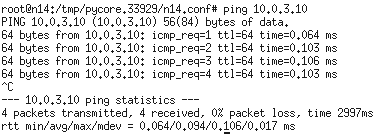
\includegraphics[width=9cm]{PARTEB_1d_n14TOsv.PNG}
\end{center}
\caption{Teste de conectividade entre departamento C e o servidor}
\end{figure}

\subsection{Questão E}
\hspace{3mm}
\questionE{Verifique se existe conectividade IP do \textit{router} de acesso Rex para o servidor S1}\\

\begin{figure}[H]
\begin{center}
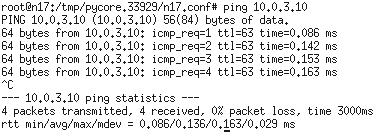
\includegraphics[width=10cm]{PARTEB_1e_routerExteriorTOsv.PNG}
\end{center}
\caption{Teste de conectividade entre \textit{router} exterior e o servidor}
\end{figure}

\clearpage

\section{Grupo II - Parte 2}

\subsection{Questão A}
\hspace{3mm} 
\questionE{Execute o comando netstat –rn por forma a poder consultar a tabela de encaminhamento unicast	(IPv4). Inclua no seu relatório as tabelas de encaminhamento obtidas; interprete as várias entradas de cada tabela. Se necessário, consulte o manual respetivo (man netstat).}\\

Por análise da figura 21 (tabela de encaminhamento de um host), verifica-se o seguinte:

\begin{enumerate}

    \item A primeira linha representa a rota por defeito (0.0.0.0). Significa que, todos os datagramas que não fazem \textit{match} com nenhum IP da coluna \textit{Destination}, devem ir para o router de acesso. Por isso, daí em diante, reencaminhamento fica a cargo do \textit{router}.
    
    \item A segunda linha trata de fazer encaminhar pacotes que sejam para a rede local. Ou seja, o próprio host trata de entregar os datagramas aos hosts que estão na mesma sub-rede, uma vez que conhece a topologia. 

\end{enumerate}

\begin{figure}[H]
\begin{center}
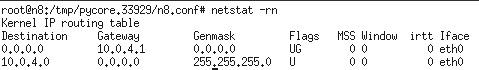
\includegraphics[width=10cm]{PARTEB_2a_tabelaN8.PNG}
\end{center}
\caption{Tabela de encaminhamento do host n8}
\end{figure}

Por análise da figura 22 (tabela de encaminhamento de um \textit{router} de acesso), verifica-se que não há rotas por defeito já que todas as rotas existentes na rede devem-se encontrar identificadas na tabela.
Então, o \textit{router} deve ser capaz de encaminhar tráfego para as redes 10.0.0.0, 10.0.1.0 e 10.0.4.0, já que em todas as linhas, o \textit{gateway} está com o valor 0.0.0.0.
Todas as restantes linhas sugerem as redes às quais o \textit{router} consegue chegar, mas às quais não está diretamente ligado. Por isso, deve reencaminhar os pacotes para os \textit{routers} que o \textit{routing} dinâmico determinou e daí a presença da \textit{flag} G no campo \textit{Flags}. 


\begin{figure}[H]
\begin{center}
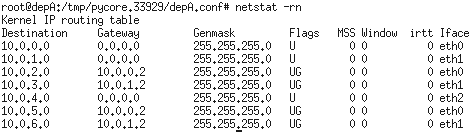
\includegraphics[width=10cm]{PARTEB_2a_tabelaRouterA.PNG}
\end{center}
\caption{Tabela de encaminhamento do \textit{router} A}
\end{figure}

\subsection{Questão B}
\hspace{3mm}
\questionE{Diga, justificando, se está a ser usado encaminhamento estático ou dinâmico (sugestão: analise que processos estão a correr em cada sistema)}\\

A partir da imagem abaixo, é possível verificar que está a ser usado o protocolo de encaminhamento OSPF.

OSPF significa \textit{Open Shortest Path First} e é um protocolo de encaminhamento dinâmico que foi criado para substituir o antigo RIP.

Conclui-se, por isso, que está a ser usado encaminhamento dinâmico e, como tal, as rotas são calculadas automaticamente.

\begin{figure}[H]
\begin{center}
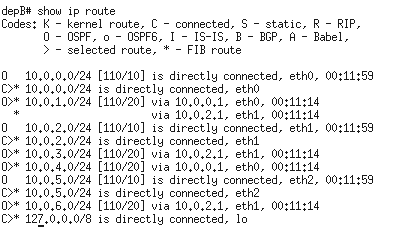
\includegraphics[width=10cm]{PARTEB_2b_OSPFrunningNoRouterB.PNG}
\end{center}
\caption{Informações de encaminhamento no \textit{router} B}
\end{figure}

\subsection{Questão C}
\hspace{3mm}
\questionE{Admita que, por questões administrativas, a rota por	defeito	(0.0.0.0 ou \textit{default}) deve	ser retirada definitivamente da tabela de encaminhamento do servidor S1 localizado no departamento C. Use o comando \textit{route delete} para o efeito. Que implicações tem esta medida para os utilizadores da empresa que acedem ao servidor. Justifique.}\\

\begin{figure}[H]
\begin{center}
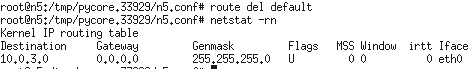
\includegraphics[width=12cm]{PARTEB_2c_rotaapagada.PNG}
\end{center}
\caption{Tabela de encaminhamento após o comando \textit{route del}}
\end{figure}

Após a remoção da rota \textit{default} ou 0.0.0.0, o \textit{router} não sabe o que fazer aos pacotes que não fazem \textit{match} com o que está na tabela de encaminhamento. 
No entanto, não se removeu da tabela o encaminhamento para a rede local e, por isso, os utilizadores do departamento continuam com conectividade, como se mostra na imagem abaixo.
Em relação a pacotes externos para o \textit{router}, este consegue recebê-los, mas não consegue responder.

\begin{figure}[H]
\begin{center}
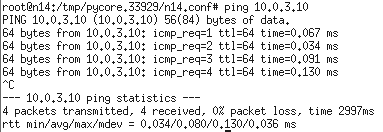
\includegraphics[width=9cm]{PARTEB_2c_n14MESMASUBREDEToSv.PNG}
\end{center}
\caption{Teste de conectividade para a rede local}
\end{figure}

\subsection{Questão D e Questão E}
\hspace{3mm}
\questionE{Adicione as rotas estáticas necessárias para restaurar a conectividade para o servidor S1,	por forma a contornar a restrição imposta na alínea c). Utilize para o efeito o comando route add e registe os comandos que usou.
Teste a nova política de encaminhamento garantindo que o servidor está novamente acessível,	utilizando para	o efeito o comando ping. Registe a nova tabela de encaminhamento do servidor.
}\\

Foram adicionadas rotas estáticas para reestabelecer a conexão entre os departamentos, estabelecendo-se que, para a rede local seria o próprio servidor a encaminhar. Para as restantes redes da topologia, seria o \textit{router} de acesso o responsável pelo encaminhamento.

Na figura 26, é possível ver os comandos usados para o efeito.

\begin{figure}[H]
\begin{center}
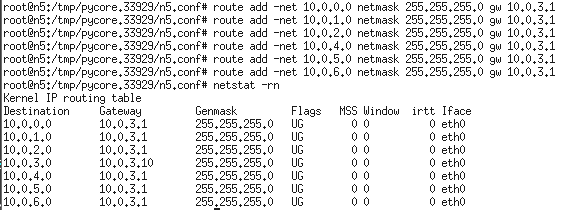
\includegraphics[width=12cm]{PARTEB_2e_tabelaErouteAdd.PNG}
\end{center}
\caption{Adição de rotas estáticas e nova tabela de encaminhamento}
\end{figure}

\begin{figure}[H]
\begin{center}
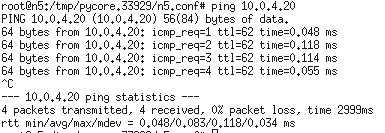
\includegraphics[width=10cm]{PARTEB_2e_ping.PNG}
\end{center}
\caption{Teste de conectividade com rota estática}
\end{figure}

\clearpage

\section{Grupo III - Parte 2}

\subsection{Questão A}
\hspace{3mm} 
\questionE{Considere que dispõe apenas do endereço de rede IP 172.XX.48.0/20, em que XX é o decimal correspondendo ao seu número de grupo (PLXX). Defina um novo esquema de endereçamento para as redes dos departamentos (mantendo a rede de acesso e core inalteradas) e atribua endereços às interfaces dos vários sistemas envolvidos. Deve justificar as opções usadas.}\\

Para a atribuição de endereços às redes dos departamentos, decidiu-se fazer subnetting.
Dos cálculos efetuados, a partir do endereço IP 172.65.48.0/20, surgiram 6 sub-redes uma vez que se usaram 3 bits para sub-redes sobrando 9 bits para hosts (12 é total de bits nos quais podemos mexer).

É importante referir que não era possível usar somente 2 bits porque ${2}^2$ = 4 e 4 - 2 = 2, que é menor que 3. 

Portanto, usando 3 bits e passando para /23, manifestaram-se 8 endereços:
\begin{itemize}
    \item 172.65.48.0/23 - DESCARTADO
    \item 172.65.50.0/23 - Sub-Rede 1
    \item 172.65.52.0/23 - Sub-Rede 2
    \item 172.65.54.0/23 - Sub-Rede 3
    \item 172.65.56.0/23 - Sub-Rede 4
    \item 172.65.58.0/23 - Sub-Rede 5
    \item 172.65.60.0/23 - Sub-Rede 6
    \item 172.65.62.0/23 - DESCARTADO
\end{itemize}

Usando então as primeiras 3 sub-redes (510 hosts em cada uma), definiu-se a seguinte topologia:

\begin{figure}[H]
\begin{center}
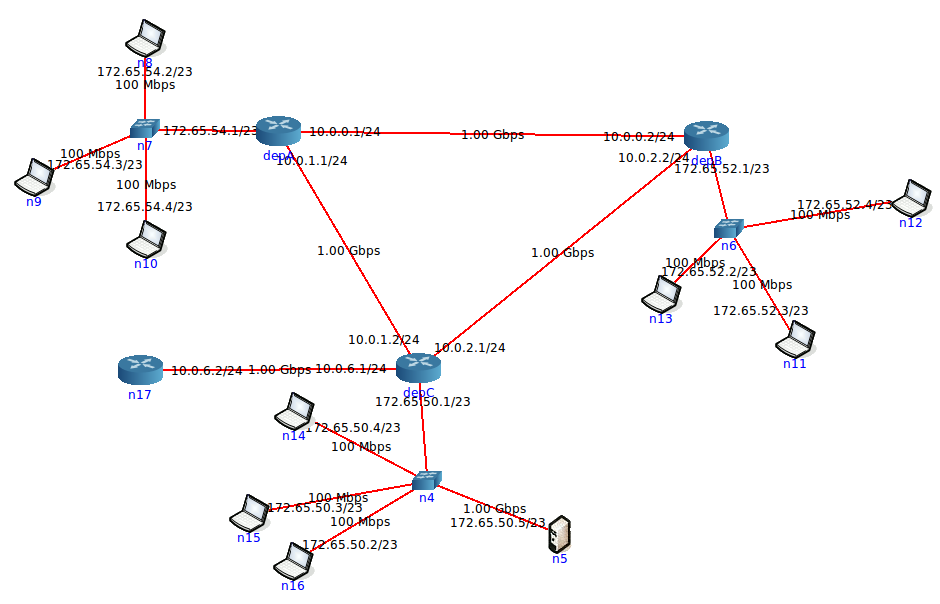
\includegraphics[width=12cm]{topoFIM.PNG}
\end{center}
\caption{Topologia da rede com \textit{subnetting}}
\end{figure}

Contudo, verifica-se nesta implementação que há um enorme desaproveitamento de espaço, já que se está a reservar espaço para sub-redes que nunca vão ser usadas no contexto do problema. Por isso, optou-se por fazer \textit{supernetting}.

Surgiu daí 3 endereços:

\begin{itemize}
    \item 172.65.50.0/23 e 172.65.52.0/23 resulta em 172.65.48.0/22
    \item 172.65.54.0/23 e 172.65.56.0/23 resulta em 172.65.52.0/22
    \item 172.65.58.0/23 e 172.65.60.0/23 resulta em 172.65.56.0/22
\end{itemize}

Ou seja, a partir do \textit{supernetting} agregando dois a dois, conseguimos ter 1022 hosts em cada sub-rede em vez dos 510 hosts iniciais.

\begin{figure}[H]
\begin{center}
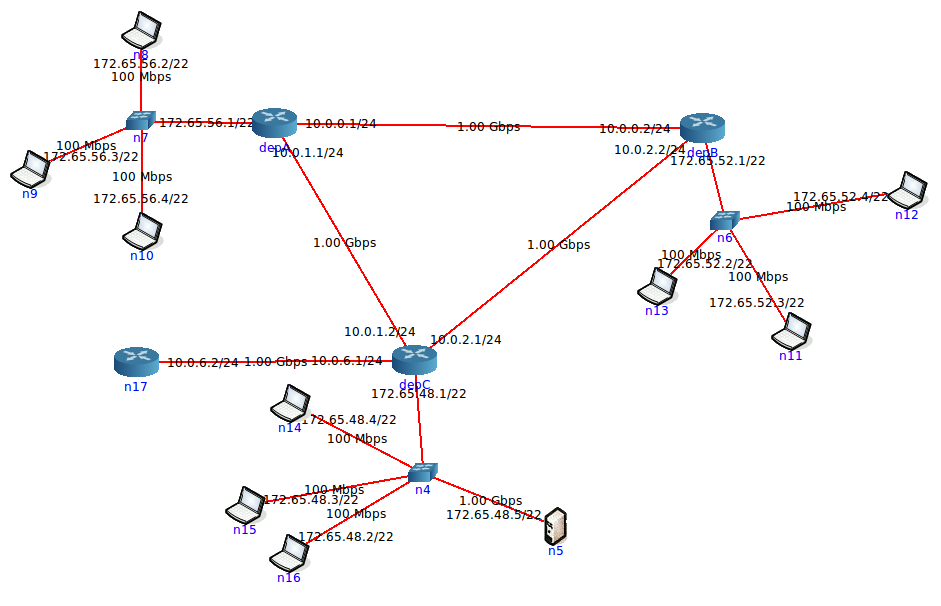
\includegraphics[width=12cm]{topoSuperN.PNG}
\end{center}
\caption{Topologia da rede com \textit{supernetting}}
\end{figure}

\subsection{Questão B}
\hspace{3mm}
\questionE{Qual a máscara de rede que usou (em formato decimal)? Quantos hosts IP pode interligar em cada departamento? Justifique.}\\

A partir do \textit{subnetting} inicial, o grupo usou um /23 que corresponde a 255.255.254.0 e, no qual, se pode interligar 510 hosts em cada departamento.
Depois, verificou-se que havia um desaproveitamento do espaço de endereçamento e, com base em \textit{supernetting}, passou-se a usar um /22 que corresponde a 255.255.252.0 e, no qual, se pode interligar 1022 hosts em cada departamento.

\subsection{Questão C}
\hspace{3mm}
\questionE{Garanta e verifique que conectividade IP entre as várias redes locais da organização	MIEI-RC é mantida. Explique como procedeu.}\\

Verifica-se há conectividade entre as várias redes locais da organização.

\begin{figure}[H]
\begin{center}
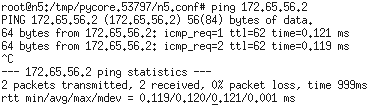
\includegraphics[width=9cm]{depCtoDepA.PNG}
\end{center}
\caption{Teste de conectividade entre departamento C e A}
\end{figure}

\begin{figure}[H]
\begin{center}
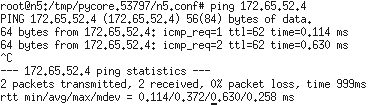
\includegraphics[width=9cm]{depCtoDepB.PNG}
\end{center}
\caption{Teste de conectividade entre departamento C e B}
\end{figure}

\begin{figure}[H]
\begin{center}
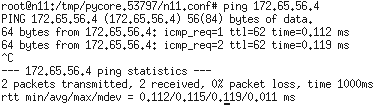
\includegraphics[width=9cm]{depBtoDepA.PNG}
\end{center}
\caption{Teste de conectividade entre departamento B e A}
\end{figure}

\section{Conclusão}
\hspace{3mm}
Neste trabalho aprofundou-se a compreensão do funcionamento interno das redes IP, principalmente nas suas estruturas e na transmissão de dados. Em particular, estudou-se o \textit{subnetting}, \textit{supernetting} e as suas aplicações bem como o potencial do \textit{routing} dinâmico e estático e a importância das tabelas de endereçamento. Em relação aos datagramas, notou-se a importância do TTL, dos diferentes protocolos IP e informações presentes tanto em \textit{headers} como em \textit{payloads}.
%BIBLIOGRAFIA


\end{document}